\chapter{Réalisation de l'application}

\section{Captures d'ecran}
\subsection{Client Mobile}
L'application se présente en plusieurs parties. Nous distinguons le panel d’authentification qui permet
à l’utilisateur de s’inscrire lors de la première utilisation et de se connecter afin d’accéder aux
autres modules de l’application. Les interfaces ci-après la présentent :
\begin{figure}[h]
    \begin{minipage}[c]{.46\linewidth}
        \centering
        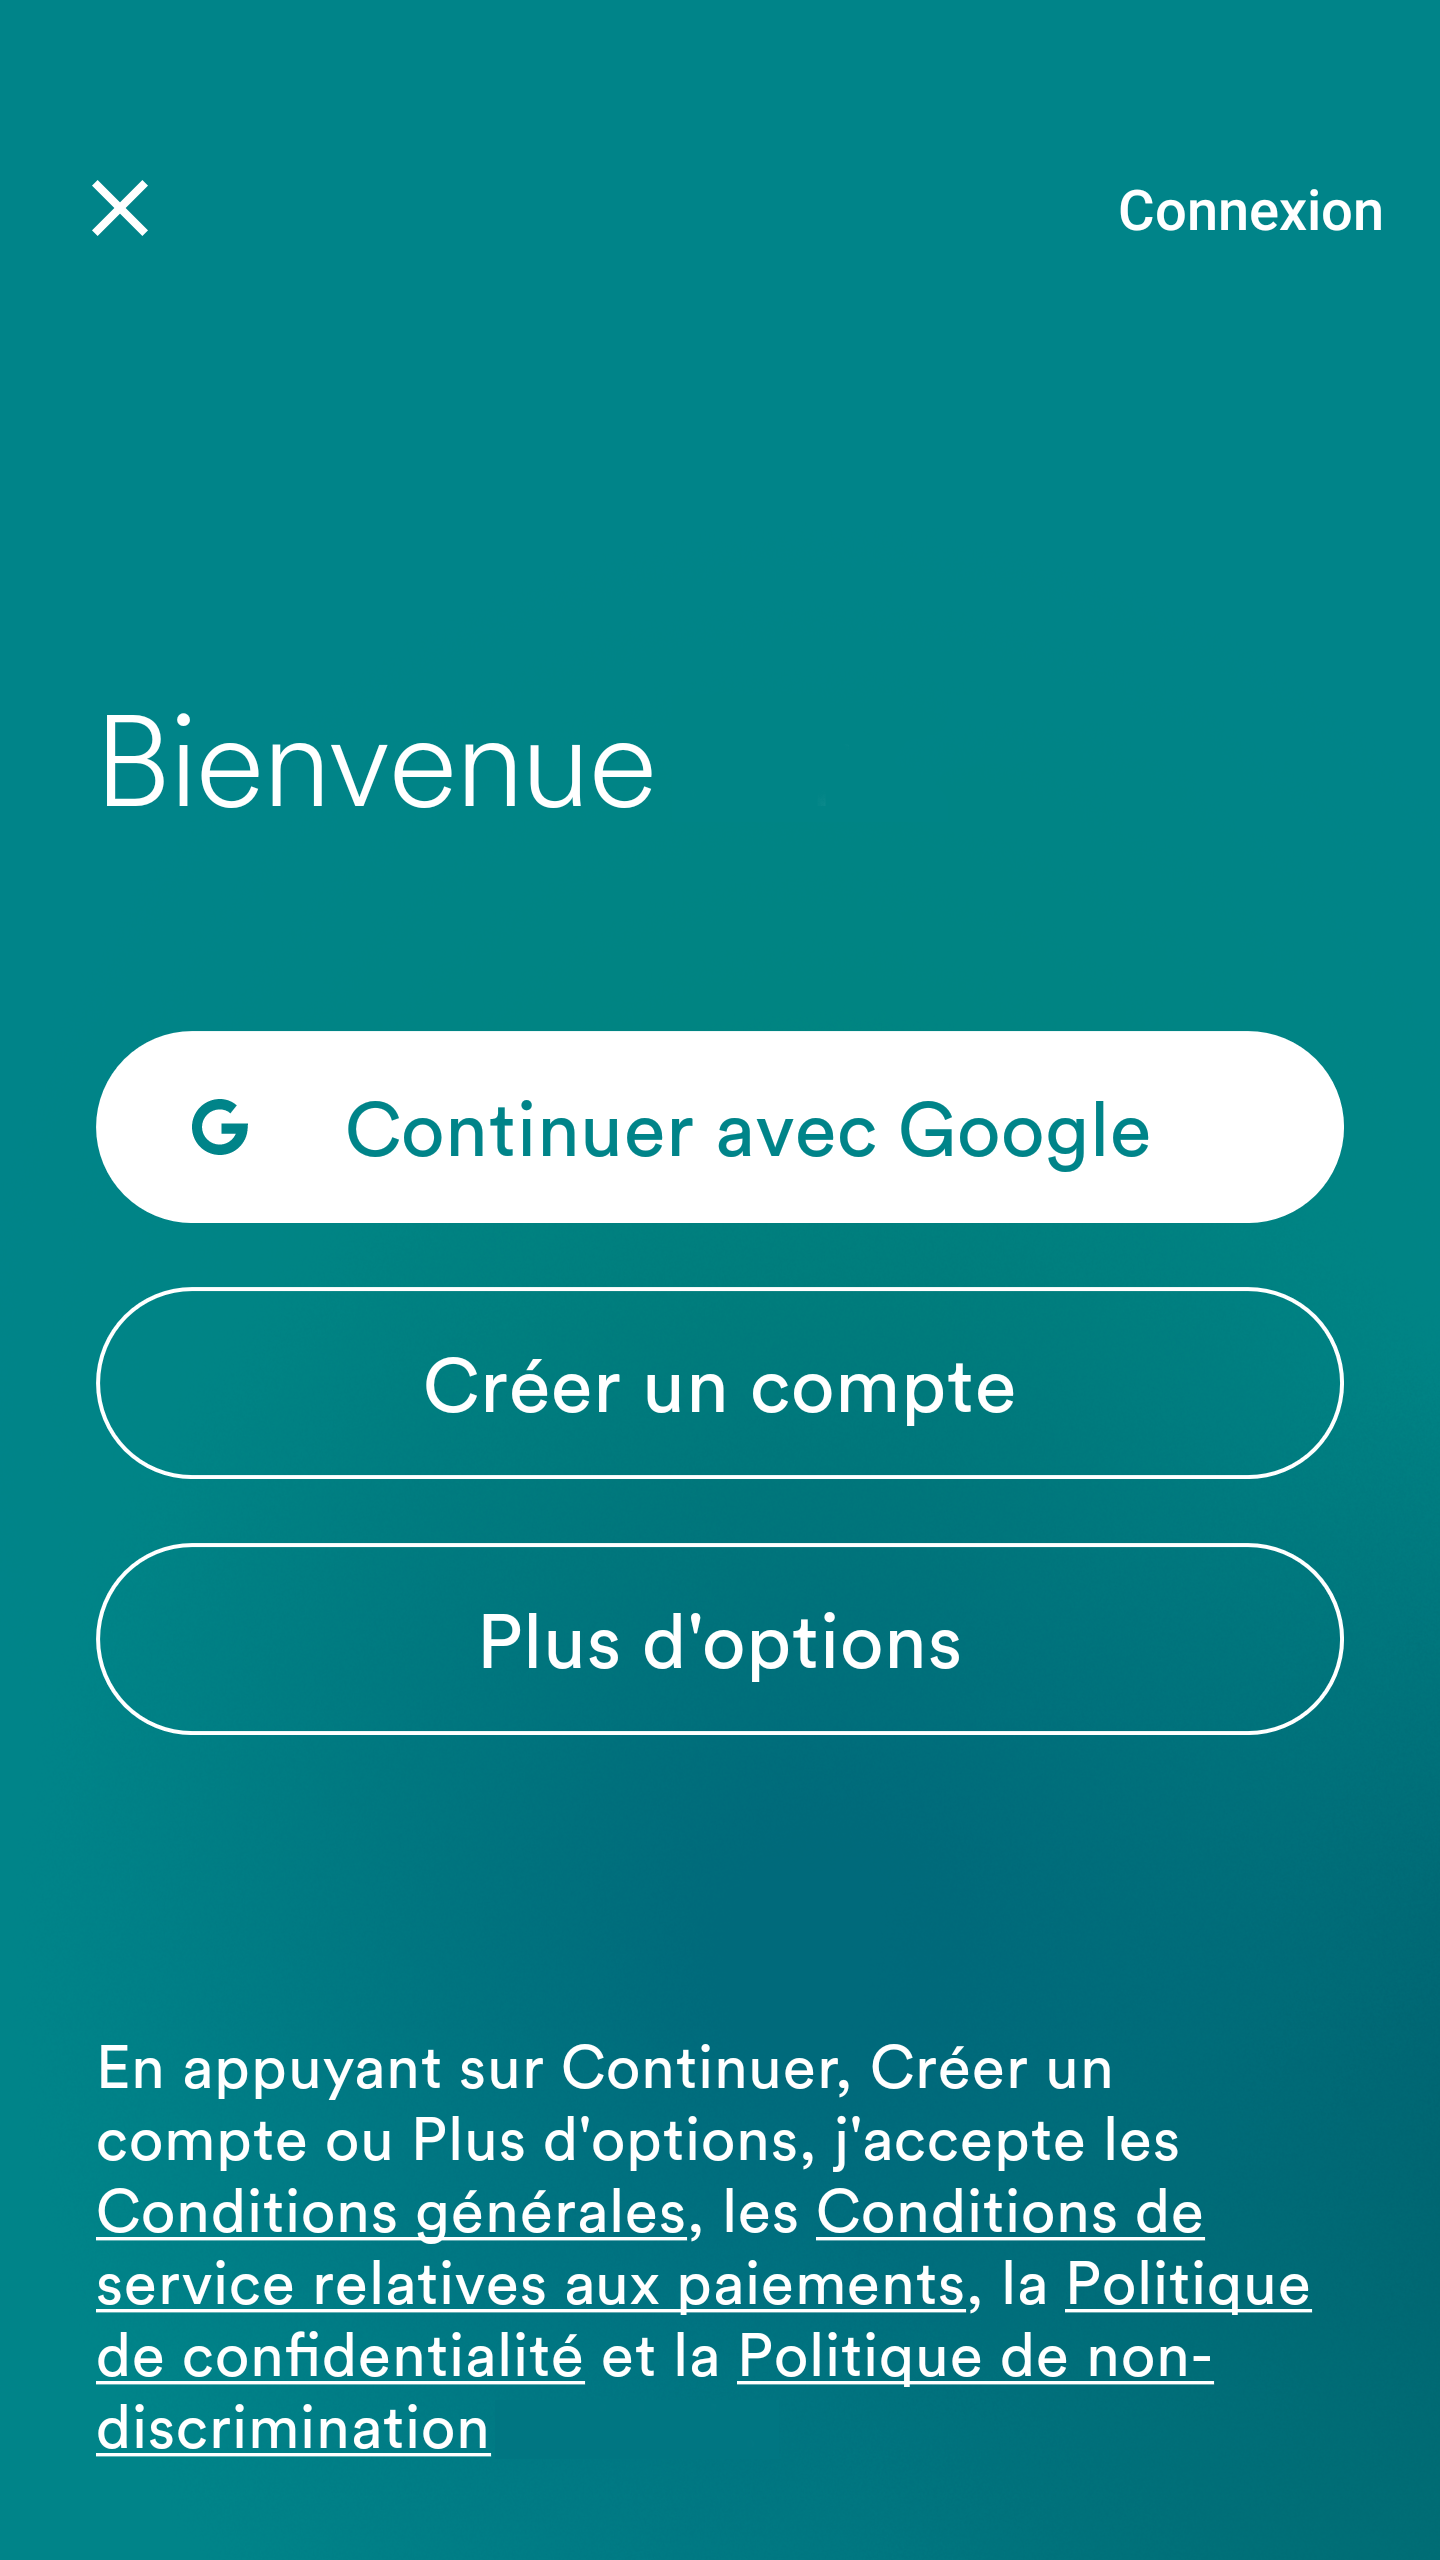
\includegraphics[width=6.5cm]{images/screen/mobile/1.png}
        \caption{Accueil - Inscription}
    \end{minipage}
    \hfill%
    \begin{minipage}[c]{.46\linewidth}
        \centering
        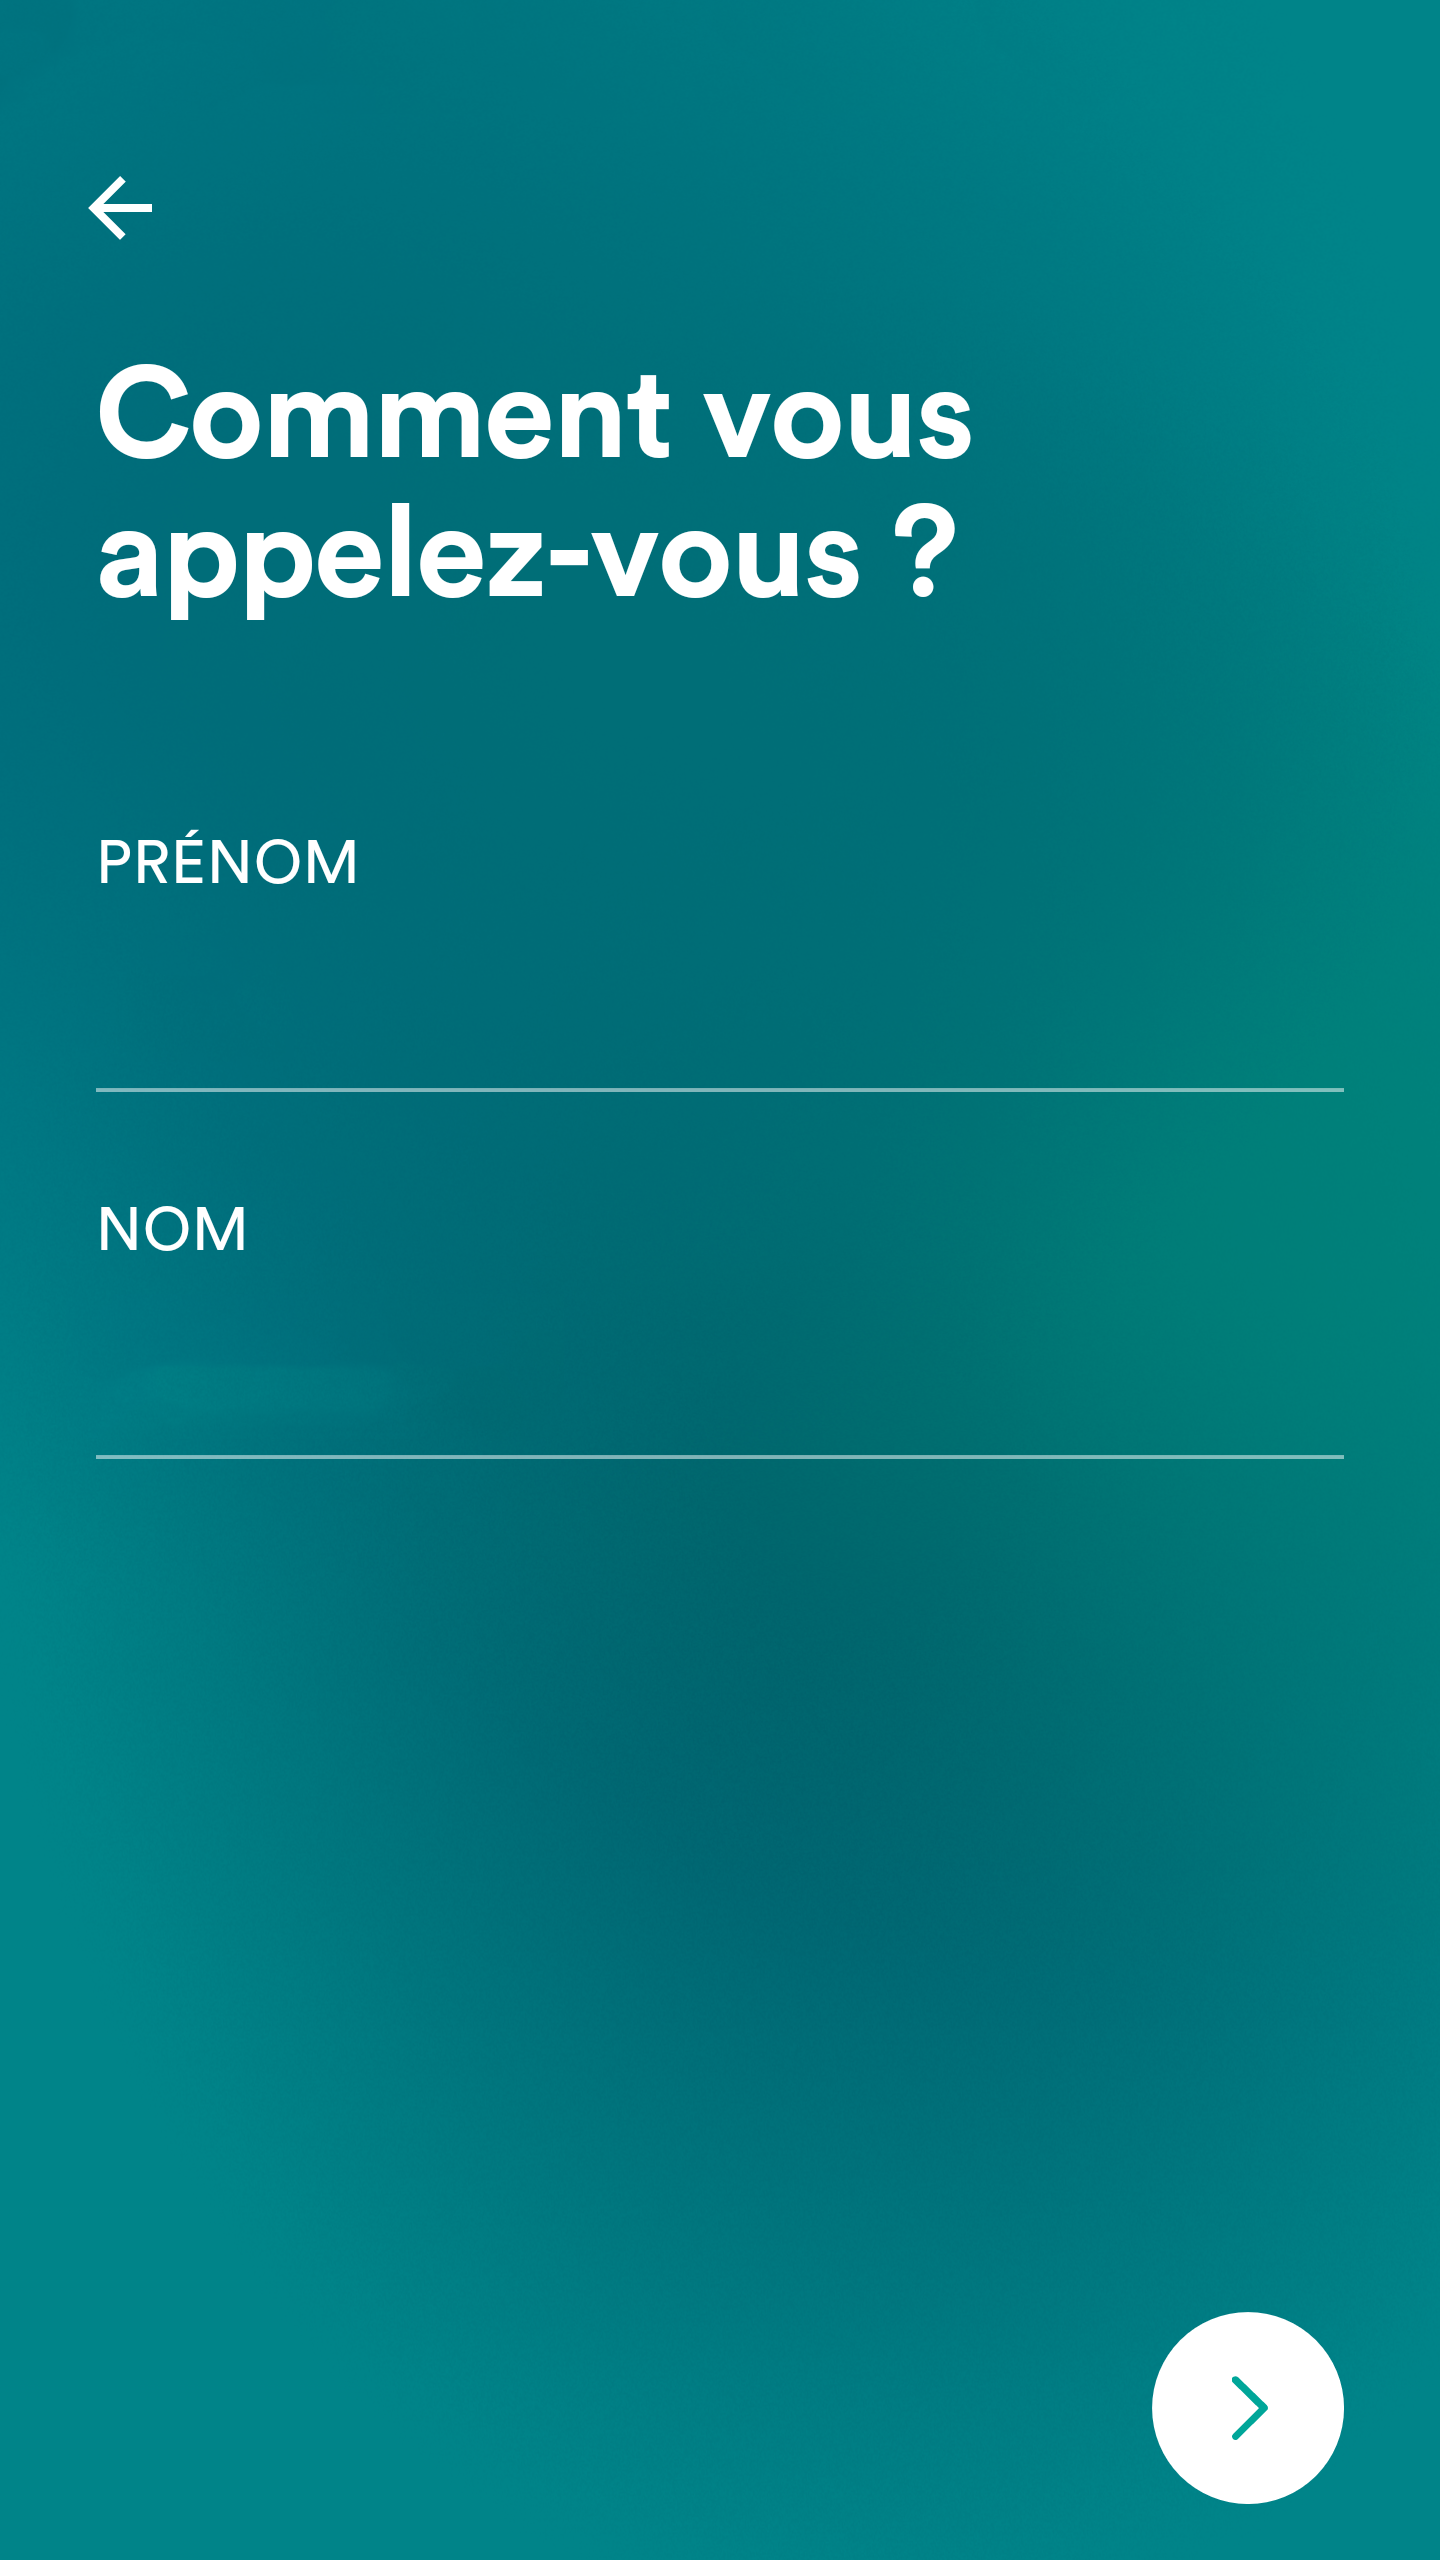
\includegraphics[width=6.5cm]{images/screen/mobile/2.png}
        \caption{Nom - Inscription}
    \end{minipage}
\end{figure}
$ $
\begin{figure}[h]
    \begin{minipage}[c]{.46\linewidth}
        \centering
        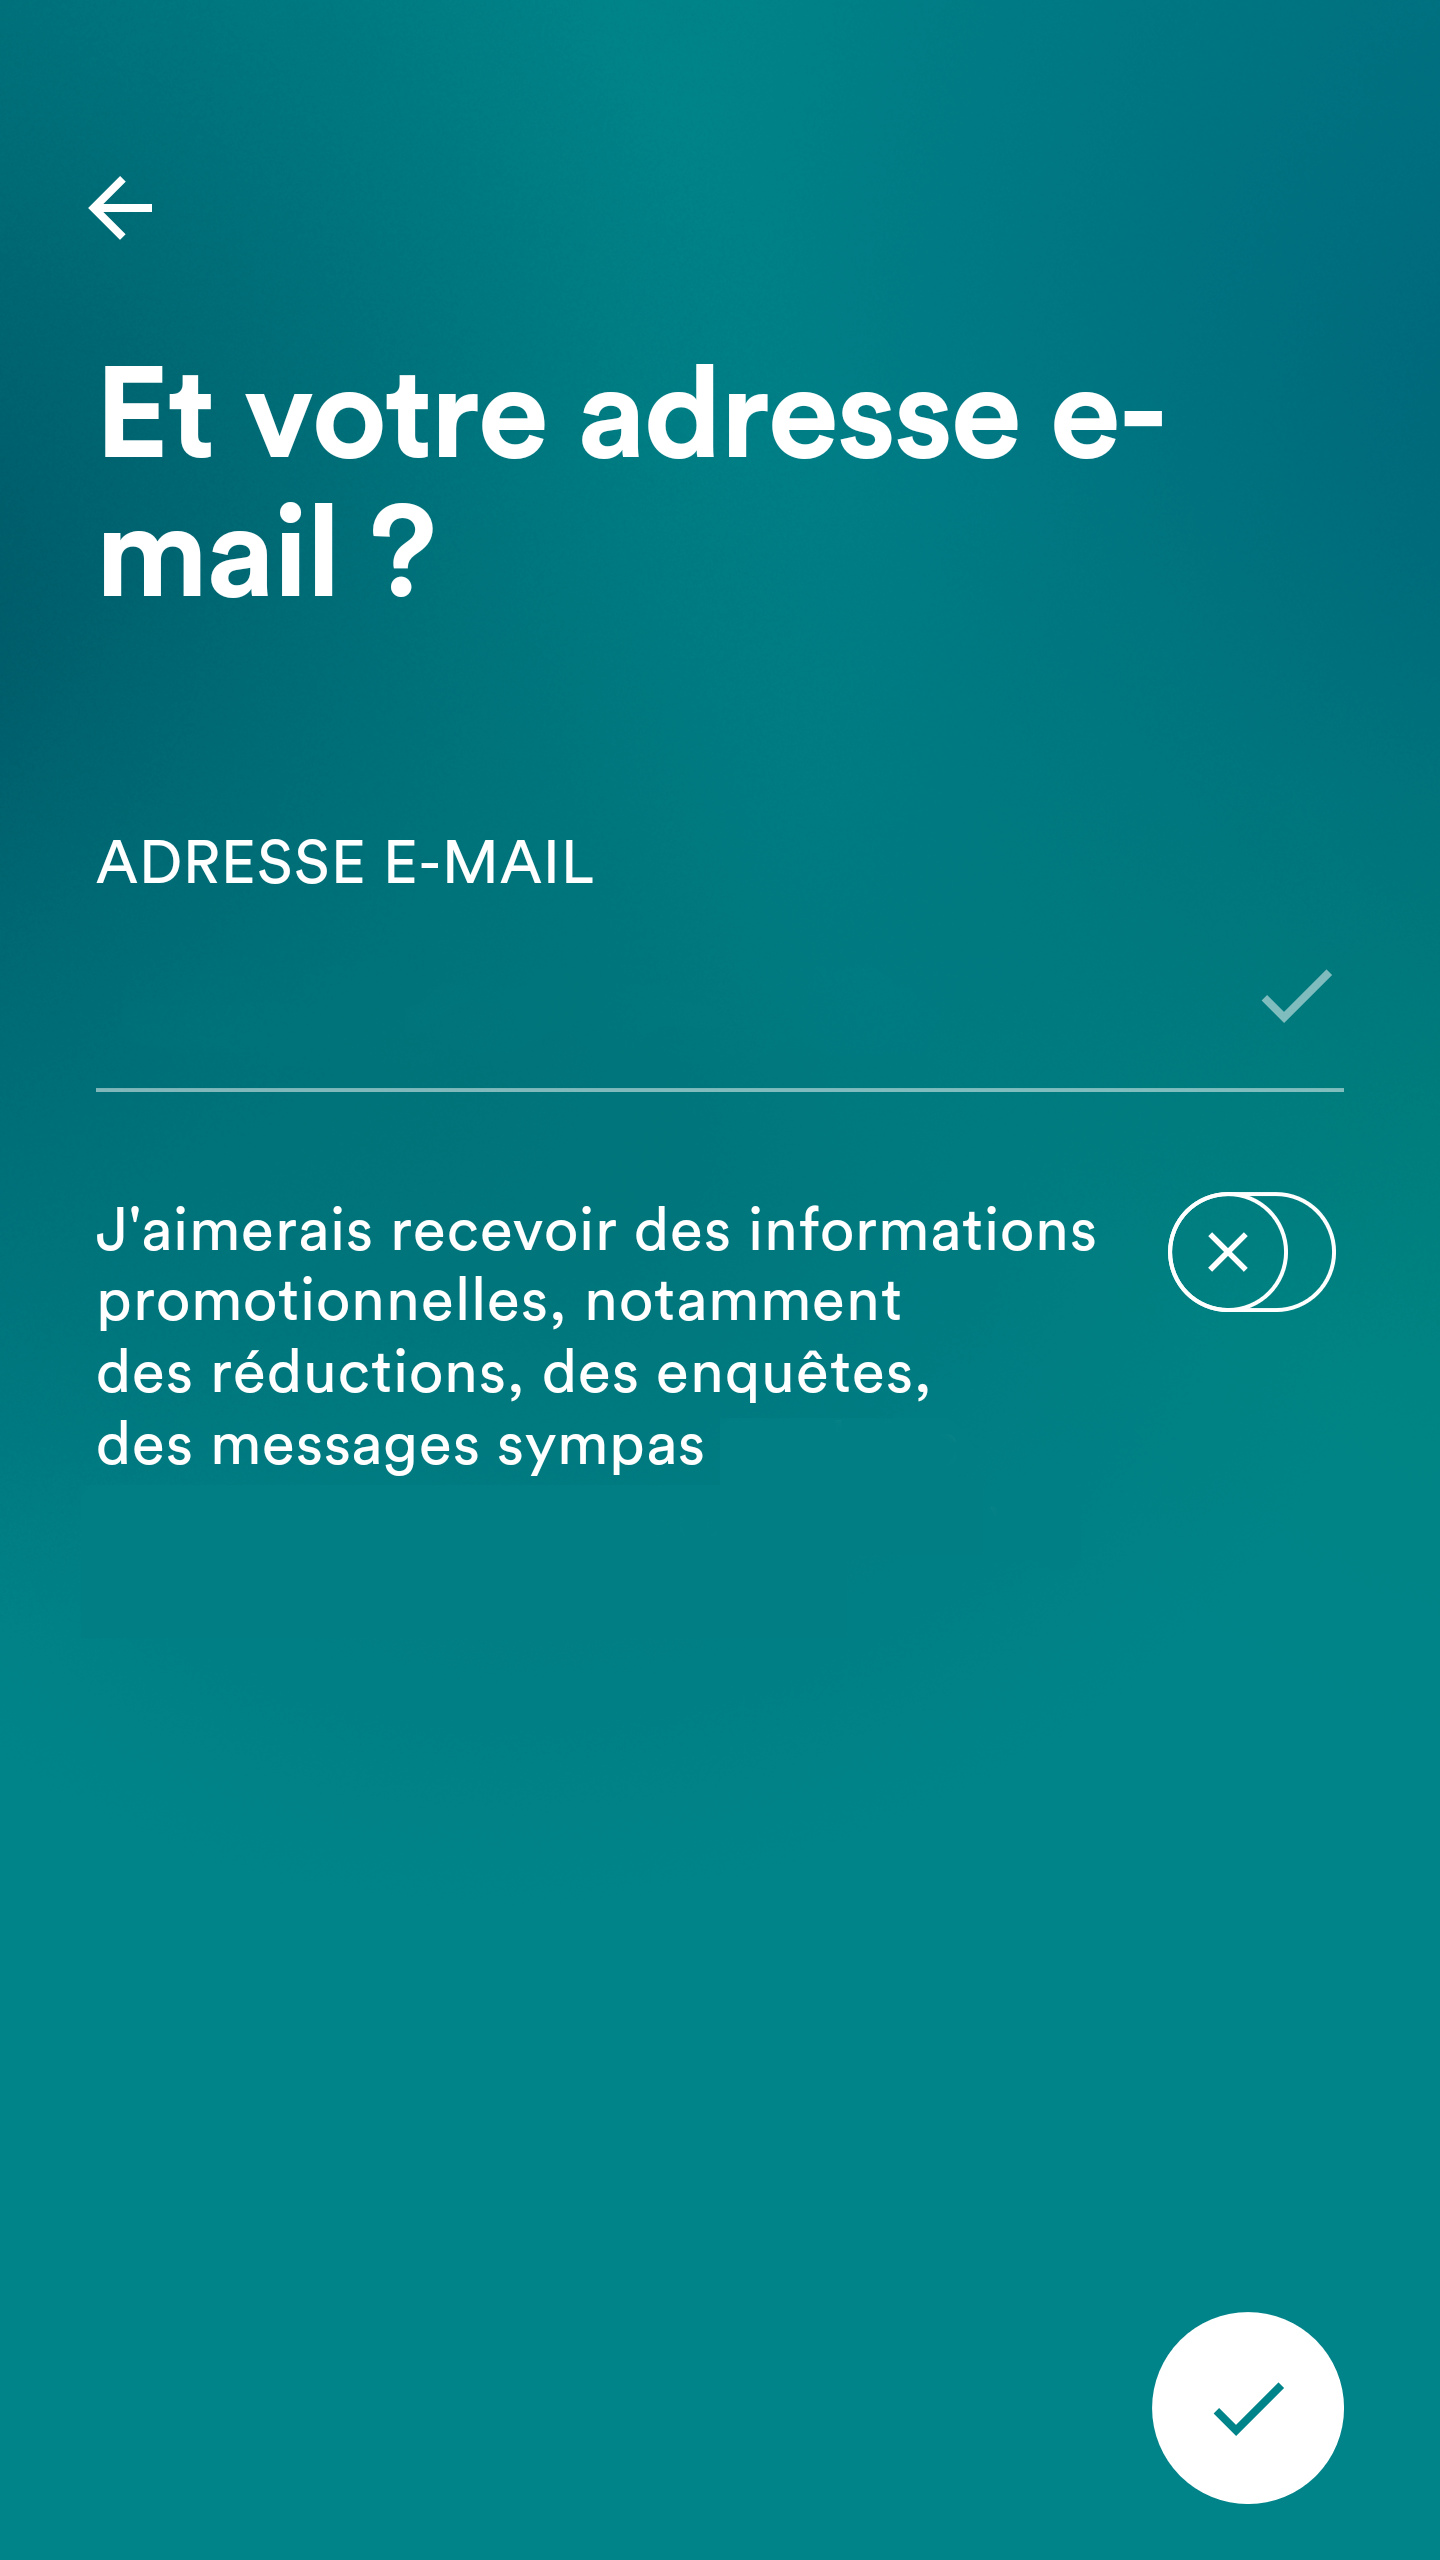
\includegraphics[width=6.5cm]{images/screen/mobile/3.png}
        \caption{Mail - Inscription}
    \end{minipage}
    \hfill%
    \begin{minipage}[c]{.46\linewidth}
        \centering
        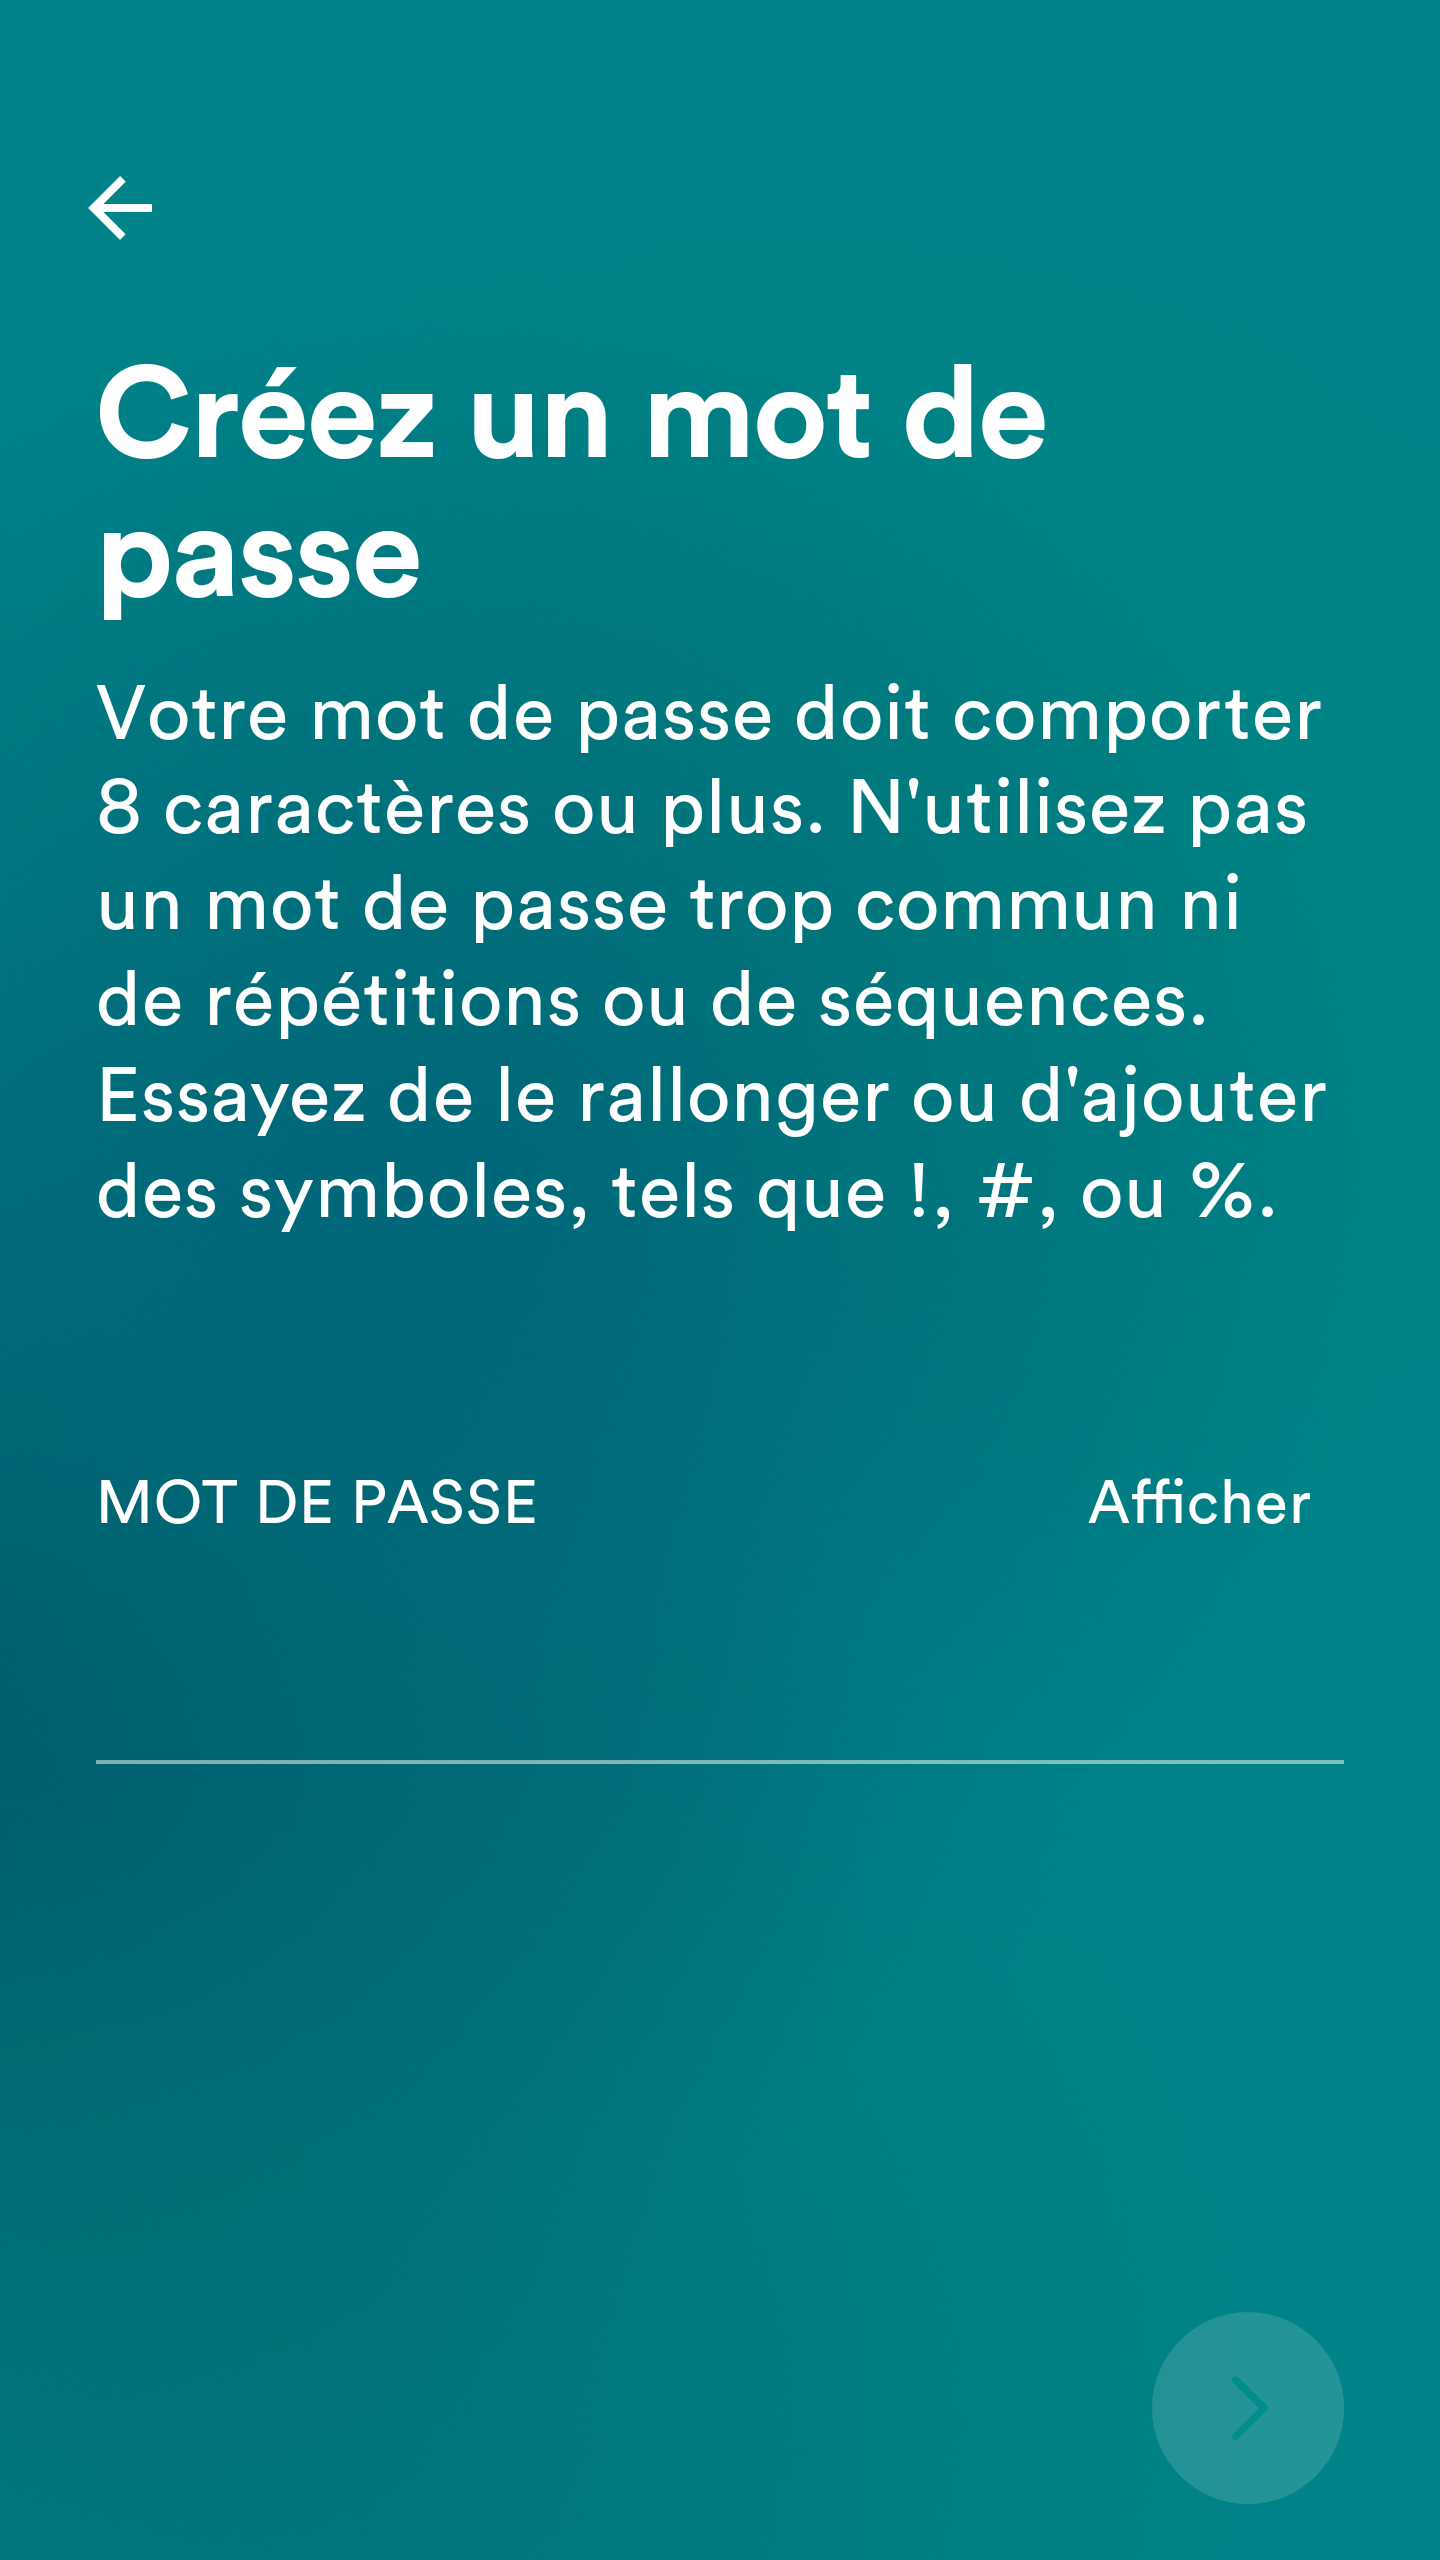
\includegraphics[width=6.5cm]{images/screen/mobile/4.png}
        \caption{Mot de passe - Inscription}
    \end{minipage}
\end{figure}

\subsection{Client Web}
\begin{figure}[H]
	\begin{center}
		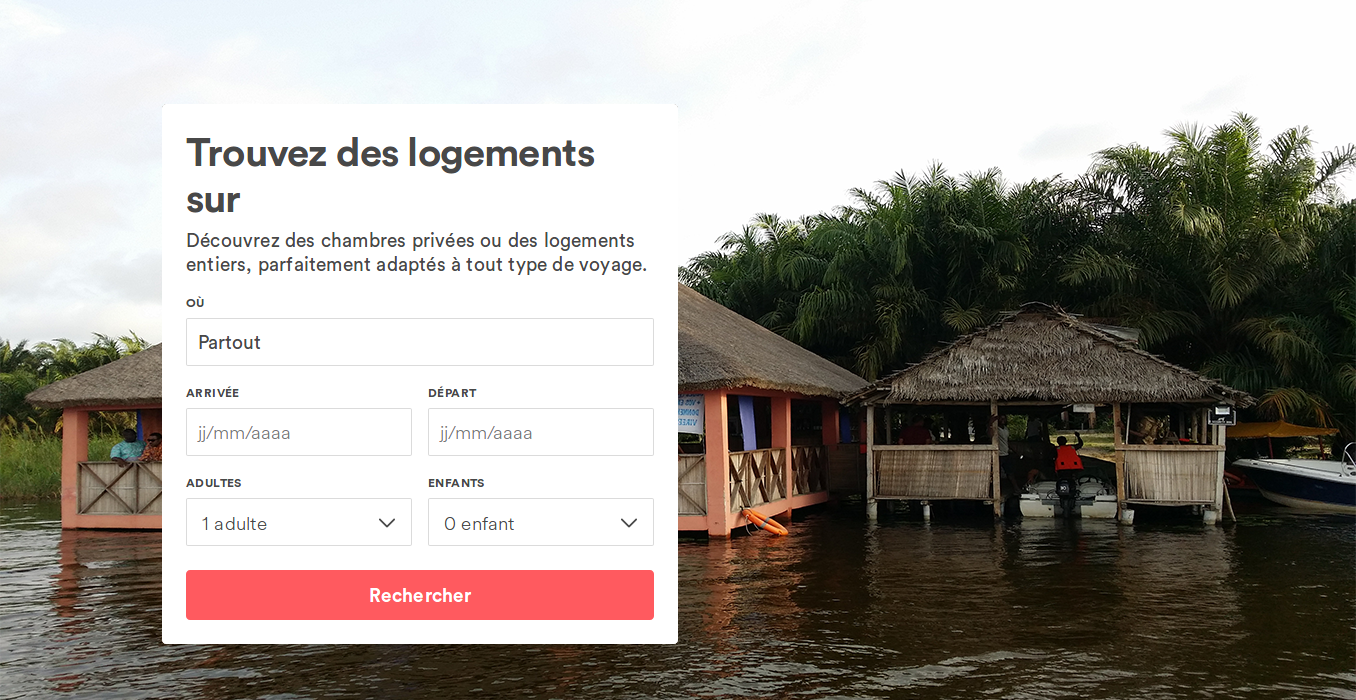
\includegraphics[width=17cm]{images/screen/web/1.png}
	\end{center}
	\caption{Accueil}
\end{figure}
\begin{figure}[H]
	\begin{center}
		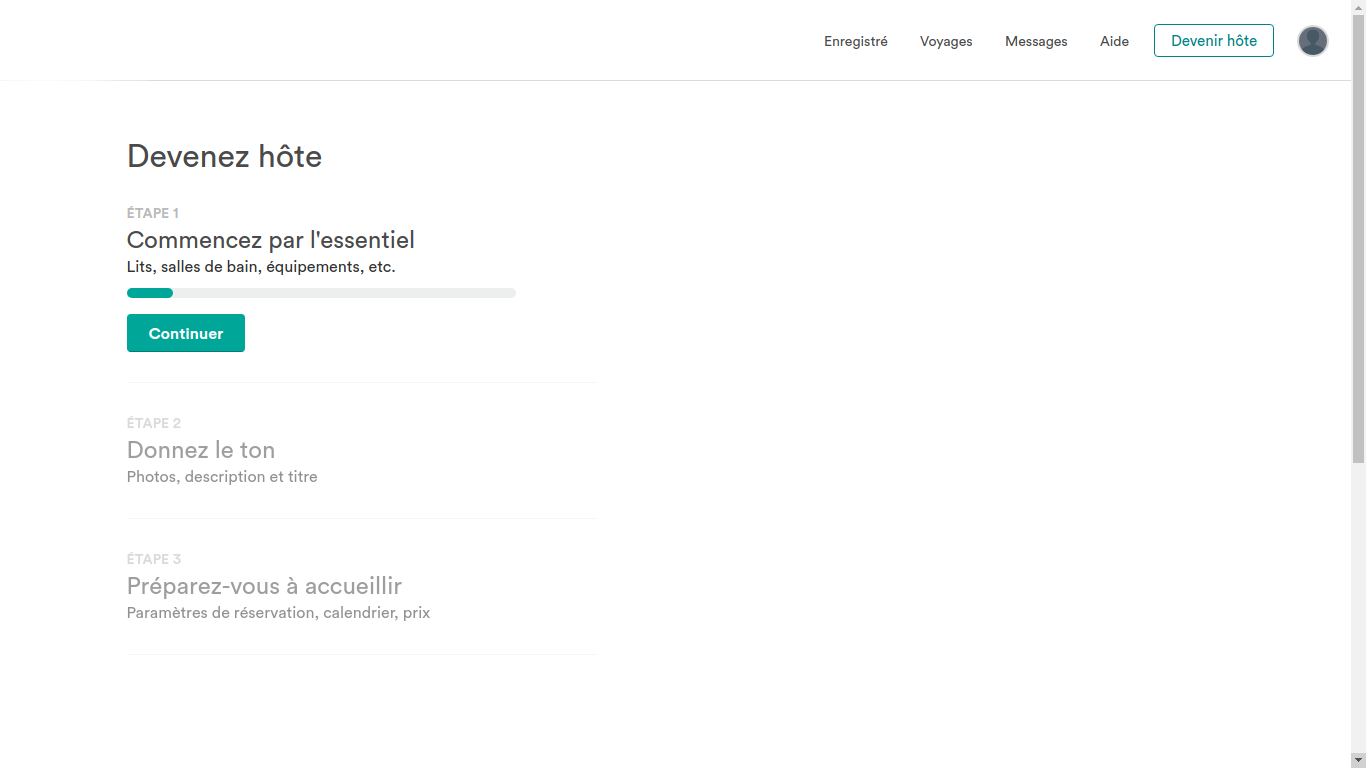
\includegraphics[width=17cm]{images/screen/web/3.png}
	\end{center}
	\caption{Devenir un hôte}
\end{figure}

\section{Déploiement de l'application}
Le déploiement de l’application et la mise en production s’est fait en continu tout au long du développement en utilisant le service Heroku\footnote{https://www.heroku.com/}.
\subsection{Heroku}
Heroku est un service de cloud computing de type PaaS\footnote{Platform-as-a-Service (plate-forme en tant que service)}. Créé en 2007, il était l'un des tout premiers services cloud. À l'origine dévolue aux applications web programmées en Ruby et utilisant Ruby on Rails, l'offre s'est ensuite étendue à d'autres runtimes : node.js, Java, Clojure, Python et Django, Scala, ainsi que PHP. Le service permet le déploiement très rapide d'applications web dans le cloud, avec une gestion très souple du scaling horizontal au travers d'un modèle de gestion des processus emprunté à Unix et adapté au Web. Côté bases de données, Heroku intègre plusieurs bases NoSQL, dont MongoDB et Redis.
L’environnement Heroku est accessible à travers la ligne de commande, via git, et un ensemble d'outils: Heroku-CLI.\\
Pour mettre en ligne les modification du projet nous avons a saisir les commandes:
\begin{lstlisting}
git add .
git commit -m 'modifications'
git push heroku master
\end{lstlisting}
Notre base de donnée est hébergée sur MongoLab un service DaaS\footnote{Database-as-a-Service}
spécialisé en hébergement MongoDB 
Ensuite nous avons essayé d'intégrer des tests (tests unitaires, tests d'intégration et tests de validation) mais cela n’a été possible faute de temps.
\\\\
Enfin nous avons acheté le nom de domaine nymeria.co ou l'application est desormais disponible.

\section{Perspectives et évolution de la plateforme}
Nous avons prévu de nombreuses améliorations pour le projet:
\begin{enumerate}
	\item Mettre en place des tests unitaires et automatiser le déploiement
	\item Achever le développement de l’API et de l'application mobile
	\item Pousser plus loin l’utilisation de React et de Redux
	\item Améliorer les algorithmes utilisés afin de faire des proposition de logement plus personnalisés et pertinentes
	\item Améliorer l’interface de l'application
	\item Intégrer les API de paiement Moov et Mtn Mobile Money
\end{enumerate}
